\documentclass[serif]{beamer}\usepackage[]{graphicx}\usepackage[]{color}
%% maxwidth is the original width if it is less than linewidth
%% otherwise use linewidth (to make sure the graphics do not exceed the margin)
\makeatletter
\def\maxwidth{ %
  \ifdim\Gin@nat@width>\linewidth
    \linewidth
  \else
    \Gin@nat@width
  \fi
}
\makeatother

\definecolor{fgcolor}{rgb}{0.345, 0.345, 0.345}
\newcommand{\hlnum}[1]{\textcolor[rgb]{0.686,0.059,0.569}{#1}}%
\newcommand{\hlstr}[1]{\textcolor[rgb]{0.192,0.494,0.8}{#1}}%
\newcommand{\hlcom}[1]{\textcolor[rgb]{0.678,0.584,0.686}{\textit{#1}}}%
\newcommand{\hlopt}[1]{\textcolor[rgb]{0,0,0}{#1}}%
\newcommand{\hlstd}[1]{\textcolor[rgb]{0.345,0.345,0.345}{#1}}%
\newcommand{\hlkwa}[1]{\textcolor[rgb]{0.161,0.373,0.58}{\textbf{#1}}}%
\newcommand{\hlkwb}[1]{\textcolor[rgb]{0.69,0.353,0.396}{#1}}%
\newcommand{\hlkwc}[1]{\textcolor[rgb]{0.333,0.667,0.333}{#1}}%
\newcommand{\hlkwd}[1]{\textcolor[rgb]{0.737,0.353,0.396}{\textbf{#1}}}%

\usepackage{framed}
\makeatletter
\newenvironment{kframe}{%
 \def\at@end@of@kframe{}%
 \ifinner\ifhmode%
  \def\at@end@of@kframe{\end{minipage}}%
  \begin{minipage}{\columnwidth}%
 \fi\fi%
 \def\FrameCommand##1{\hskip\@totalleftmargin \hskip-\fboxsep
 \colorbox{shadecolor}{##1}\hskip-\fboxsep
     % There is no \\@totalrightmargin, so:
     \hskip-\linewidth \hskip-\@totalleftmargin \hskip\columnwidth}%
 \MakeFramed {\advance\hsize-\width
   \@totalleftmargin\z@ \linewidth\hsize
   \@setminipage}}%
 {\par\unskip\endMakeFramed%
 \at@end@of@kframe}
\makeatother

\definecolor{shadecolor}{rgb}{.97, .97, .97}
\definecolor{messagecolor}{rgb}{0, 0, 0}
\definecolor{warningcolor}{rgb}{1, 0, 1}
\definecolor{errorcolor}{rgb}{1, 0, 0}
\newenvironment{knitrout}{}{} % an empty environment to be redefined in TeX

\usepackage{alltt}
\usetheme{Boadilla}
\usetheme{Boadilla}
\usepackage{graphicx}
\usepackage[final]{animate}
\usepackage{breqn}
\usepackage{xcolor}
\usepackage{booktabs}
\usepackage{tikz}
\usetikzlibrary{decorations.pathreplacing}
\usetikzlibrary{shapes,arrows,positioning,shadows}
\definecolor{links}{HTML}{2A1B81}
\hypersetup{colorlinks,linkcolor=links,urlcolor=links}
\usepackage{subfig}
\usepackage{pgf}

% knitr and global options


% load R libraries


% custom colors, do not cache
\definecolor{mypal1}{HTML}{EDF8FB}\definecolor{mypal2}{HTML}{B2E2E2}\definecolor{mypal3}{HTML}{66C2A4}\definecolor{mypal4}{HTML}{2CA25F}\definecolor{mypal5}{HTML}{006D2C}

% my custom ggplot theme


% colors and macros
\setbeamercolor{title}{fg=mypal5} % main title
\setbeamercolor{frametitle}{fg=mypal4, bg=mypal2} % frame titles
\setbeamercolor{structure}{fg=mypal4} % bottom banner
\setbeamercolor{normal text}{fg=mypal5}
\usebackgroundtemplate{
\includegraphics[height=\paperheight,width=\paperwidth]{fig/back_tmp.pdf}}

\tikzstyle{block} = [rectangle, draw, text width=9em, text centered, rounded corners, minimum height=3em, minimum width=7em, top color = white, bottom color=brown!30,  drop shadow]

\newcommand{\ShowSexpr}[1]{\texttt{{\char`\\}Sexpr\{#1\}}}

\newcommand{\Bigtxt}[1]{\textbf{\textit{#1}}}

\setbeamertemplate{enumerate items}[circle]
\IfFileExists{upquote.sty}{\usepackage{upquote}}{}
\begin{document}

\title[SWMPr for estuarine time series]{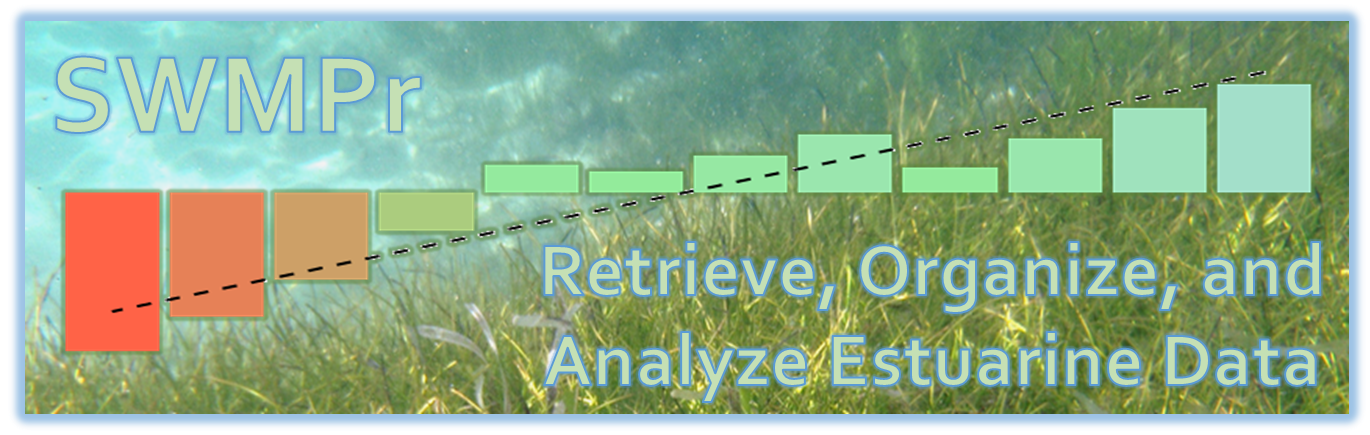
\includegraphics[width=0.85\textwidth]{fig/swmpr_logo.png}}

\author[M. Beck]{Marcus W. Beck}

\date{May 8, 2015}

\institute[]{ORISE, USEPA NHEERL Gulf Ecology Division\\ Phone: 8509342480, Email: \href{mailto:beck.marcus@epa.gov}{beck.marcus@epa.gov}}

%%%%%%
\begin{frame}
\titlepage
\end{frame}

\section{Background}

%%%%%%
\begin{frame}{Overview}
\begin{itemize}
\item What is NERRS/SWMP and motivation for creating the package \\~\\
\item What can SWMPr do \\~\\
\item What has SWMPr done \\~\\
\item How I can help, questions for the group
\end{itemize}
\end{frame}

%%%%%%
\begin{frame}{What is NERRS/SWMP?}{}
{\bf NERRS}\\
National Estuarine Research Reserve System, established by Coastal Zone Management Act of 1972. Focus on \Bigtxt{long-term research}, \Bigtxt{monitoring}, \Bigtxt{education}, and \Bigtxt{stewardship} for more effective coastal management.\\~\\
{\bf SWMP}\\
System Wide Monitoring Program, initiated in 1995 to provide \Bigtxt{continuous monitoring} data at over 140 stations in each of the 28 NERRS reserves \\~\\
\end{frame}

%%%%%%
\begin{frame}{What is NERRS/SWMP?}
\centerline{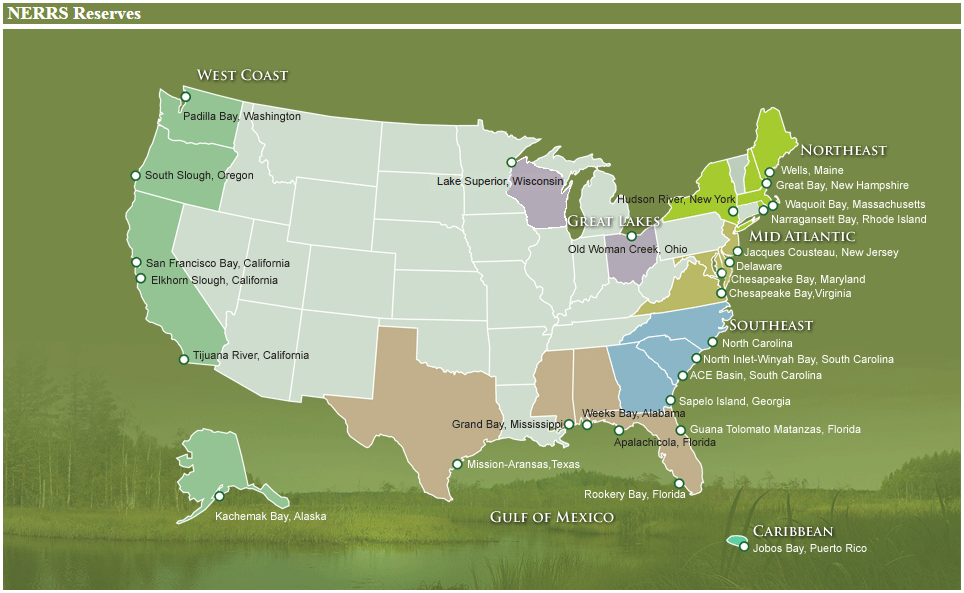
\includegraphics[width = 0.9\textwidth]{fig/NERRS_locations.png}}
\tiny
\flushright
\href{http://nerrs.noaa.gov/ReservesMap.aspx}{http://nerrs.noaa.gov/ReservesMap.aspx}
\end{frame}

%%%%%%
\begin{frame}{What is NERRS/SWMP?}
Each reserve has fixed, continuous monitoring stations for \Bigtxt{water quality} (15 min), \Bigtxt{meteorology} (15 min), and \Bigtxt{nutrients} (monthly)\\~\\
The parameters for a station are specific to the parameter type \\~\\
\begin{columns}[t]
\begin{column}{0.3\textwidth}
\Bigtxt{Water quality} \\~\\
temp, spcond, sal, do\_pct, do\_mgl, depth, cdepth, level, clevel, ph, turb, chlfluor
\end{column}
\begin{column}{0.3\textwidth}
\Bigtxt{Meteorology} \\~\\
atemp, rh, bp, wspd, maxwspd, wdir, sdwdir, totpar, totprcp, cumprcp, totsorad \\~\\
\end{column}
\begin{column}{0.3\textwidth}
\Bigtxt{Nutrients} \\~\\
po4f, chla\_n, no3f, no2f, nh4f, no23f, ke\_n, urea
\end{column}
\end{columns}
\end{frame}

%%%%%%
\begin{frame}[t]{What is NERRS/SWMP?}
Data maintained by the Centralized Data Management Office (\href{http://cdmo.baruch.sc.edu/}{CDMO})\\~\\
\centerline{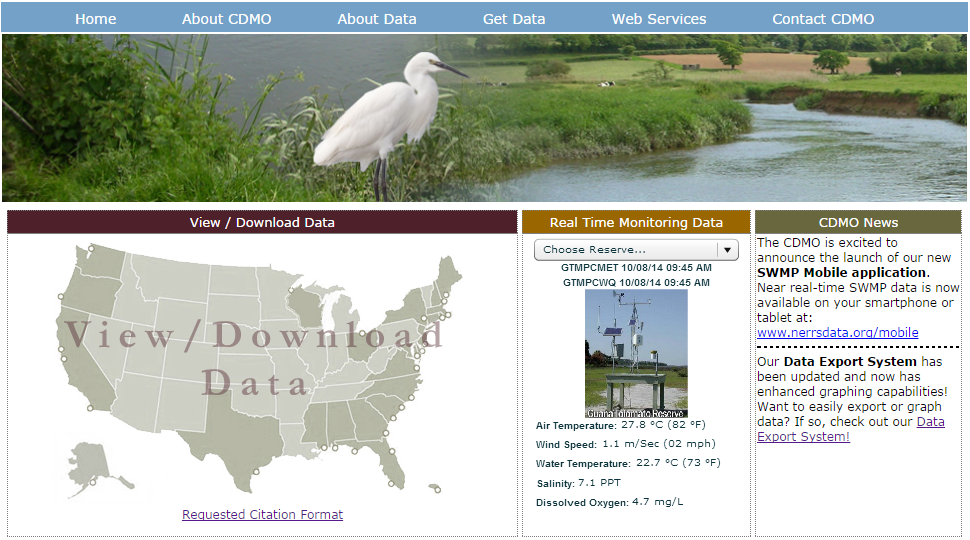
\includegraphics[width = \textwidth]{fig/cdmo_front.png}}
\end{frame}

%%%%%%
\begin{frame}{What is NERRS/SWMP?}
CDMO is an existing data management infrastructure for SWMP, services include:\\~\\
\begin{itemize}
\item Automated QAQC \\~\\
\item Numerous data download options \\~\\
\item Web services/API for remote data retrieval \\~\\
\item Simple viz tools \\~\\
\end{itemize}
\end{frame}

%%%%%%
\begin{frame}[t]{What is NERRS/SWMP?}
As of May 1, $>$ 58 million SWMP data records available from CDMO\\~\\
Raw data will look like this...\\~\\
\centerline{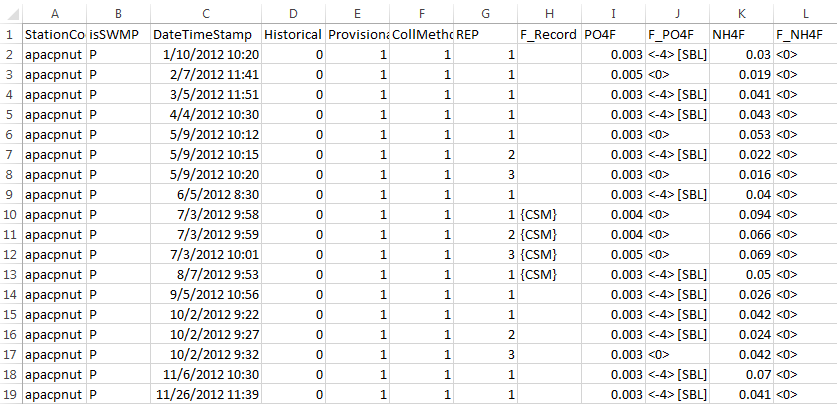
\includegraphics[width = 0.9\textwidth]{fig/qaqc_ex.png}}
\end{frame}

%%%%%%
\begin{frame}{What is the problem?}
An invaluable data source but no recent comparative analyses between systems \\~\\
NERRS researchers, managers, and technicians need more tools for trend analysis \\~\\
Some specific issues:\\~\\
\begin{itemize}
\item Knowing what data to use and how to obtain
\item Dealing with QAQC columns or removing `bad' observations
\item Combining data for comparison
\item Issues inherent with time series, e.g., signal vs. noise, data quantity
\item ...and analysis
\end{itemize}
\end{frame}

\section{SWMPr description}

%%%%%%
\begin{frame}[fragile]{What is the (potential) solution?}
\centerline{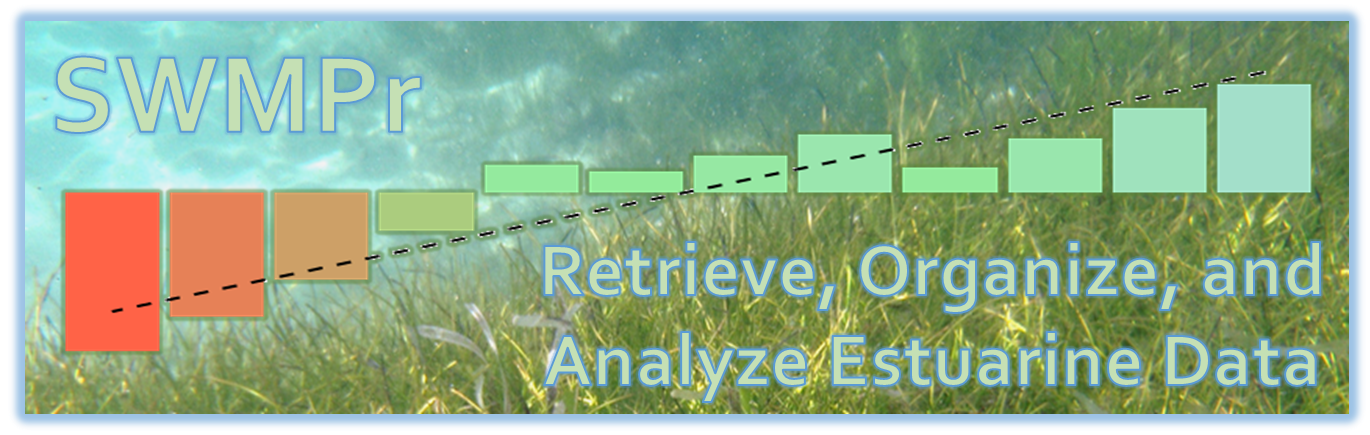
\includegraphics[width = 0.8\textwidth]{fig/swmpr_logo.png}}
\vspace{0.15in}
SWMPr v2.0.0 is officially released!
\begin{knitrout}
\definecolor{shadecolor}{rgb}{0.929, 0.973, 0.984}\color{fgcolor}\begin{kframe}
\begin{alltt}
\hlstd{> }\hlkwd{install.packages}\hlstd{(}\hlstr{'SWMPr'}\hlstd{)}
\hlstd{> }\hlkwd{library}\hlstd{(SWMPR)}
\end{alltt}
\end{kframe}
\end{knitrout}
Still in development, currently on v2.0.5
\end{frame}

%%%%%%
\begin{frame}[fragile]{SWMPr is fully documented}
\centerline{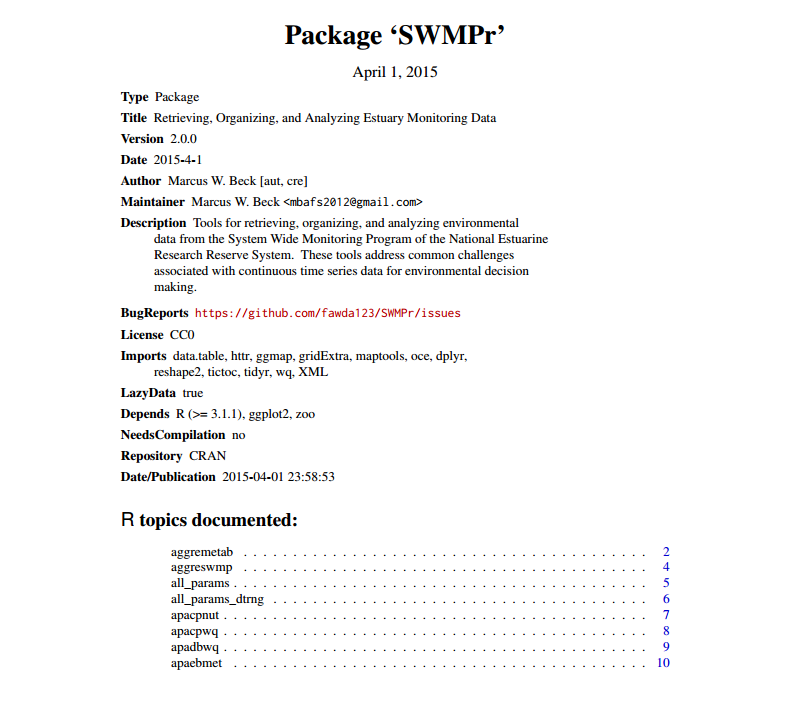
\includegraphics[width = 0.75\textwidth]{fig/swmpr_manual.png}}
\end{frame}

%%%%%%
\begin{frame}[fragile]{SWMPr is fully documented}
\centerline{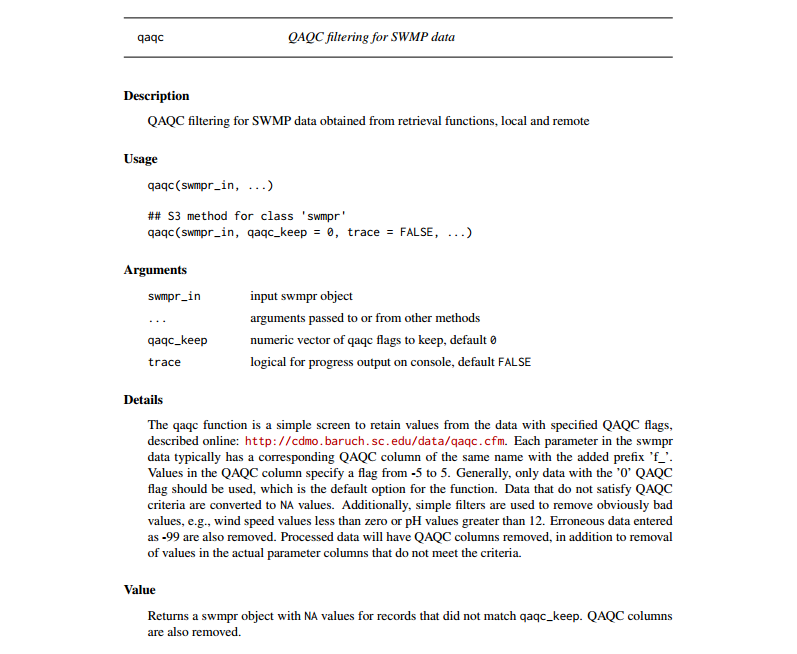
\includegraphics[width = 0.75\textwidth]{fig/help_ex.png}}
\end{frame}

%%%%%%
\begin{frame}[t]{What can SWMPr do?}
SWMPr functions are grouped into three categories that describe their use in the `data workflow'
\begin{center}
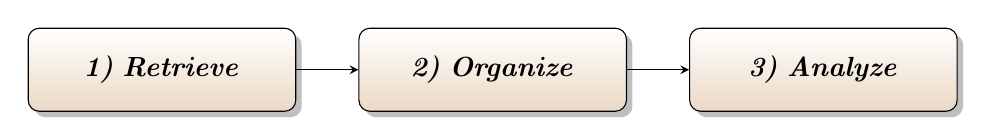
\begin{tikzpicture}[node distance=2.5cm, auto, >=stealth]
	\node[block] (a) {\Bigtxt{1) Retrieve}};
	\node[block] (b)  [right of=a, node distance=4.2cm] {\Bigtxt{2) Organize}};
 	\draw[->] (a) -- (b);
 	\node[block] (c)  [right of=b, node distance=4.2cm]  {\Bigtxt{3) Analyze}};
 	\draw[->] (b) -- (c);
\end{tikzpicture}
\end{center}
\begin{columns}[t]
\begin{column}{0.3\textwidth}
\small{
\begin{itemize}
\item Retrieve metadata \\~\\
\item Import from CDMO into R
\end{itemize}
}
\end{column}
\begin{column}{0.3\textwidth}
\small{
\begin{itemize}
\item Manipulate data for analysis \\~\\
\item Functions to clean, combine, change time step, etc.
\end{itemize}
}
\end{column}
\begin{column}{0.3\textwidth}
\small{
\begin{itemize}
\item Generic to specific applications\\~\\
\item Visualization and graphics
\end{itemize}
}
\end{column}
\end{columns}
\end{frame}

%%%%%%
\begin{frame}[fragile]{What can SWMPr do?}
Function types are searchable in R:
\begin{knitrout}
\definecolor{shadecolor}{rgb}{0.929, 0.973, 0.984}\color{fgcolor}\begin{kframe}
\begin{alltt}
\hlstd{> }\hlkwd{help.search}\hlstd{(}\hlstr{'analyze'}\hlstd{,} \hlkwc{package} \hlstd{=} \hlstr{'SWMPr'}\hlstd{)}
\end{alltt}
\end{kframe}
\end{knitrout}
\centerline{\fbox{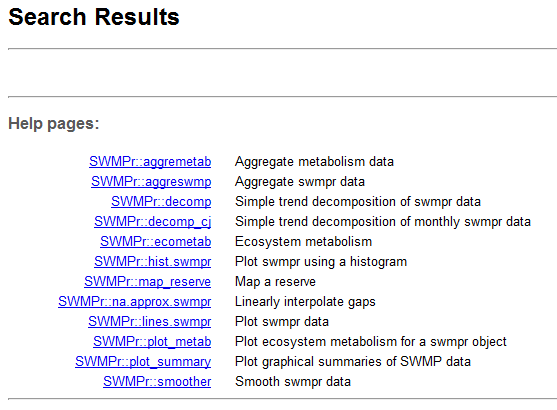
\includegraphics[width = 0.6\textwidth]{fig/searches.png}}}
\end{frame}

%%%%%%
\begin{frame}{How are data \Bigtxt{retrieved}?}
SWMPr functions can be used to import data into R three ways\\~\\
\begin{enumerate}
\item Import from a local path \\~\\
\item Retrieve SWMP data from a \href{https://s3.amazonaws.com/swmpalldata/}{third-party server} \\~\\
\item Call the existing CDMO \href{http://cdmo.baruch.sc.edu/webservices.cfm}{web services} to import directly\\~\\
\end{enumerate}
Multiple options to accommodate different types of users
\end{frame}

%%%%%%
\begin{frame}[fragile,t,shrink]{How are data \Bigtxt{retrieved}?}
The end result is the same - data are imported as a \texttt{swmpr} data object
\begin{knitrout}\small
\definecolor{shadecolor}{rgb}{0.929, 0.973, 0.984}\color{fgcolor}\begin{kframe}
\begin{alltt}
\hlstd{> }\hlstd{dat} \hlkwb{<-} \hlkwd{import_remote}\hlstd{(}\hlstr{'kacsswq'}\hlstd{)}
\hlstd{> }\hlkwd{class}\hlstd{(dat)}
\end{alltt}
\begin{verbatim}
## [1] "swmpr"      "data.frame"
\end{verbatim}
\begin{alltt}
\hlstd{> }\hlkwd{head}\hlstd{(dat,} \hlnum{1}\hlstd{)}
\end{alltt}
\begin{verbatim}
##   datetimestamp temp spcond sal do_pct do_mgl depth cdepth
## 1    2004-01-01    2     42  26    101     12   0.7     NA
##   level clevel ph turb chlfluor
## 1    NA     NA  8    6       NA
\end{verbatim}
\begin{alltt}
\hlstd{> }\hlkwd{names}\hlstd{(}\hlkwd{attributes}\hlstd{(dat))}
\end{alltt}
\begin{verbatim}
## [1] "names"       "row.names"   "class"       "station"    
## [5] "parameters"  "qaqc_cols"   "date_rng"    "timezone"   
## [9] "stamp_class"
\end{verbatim}
\end{kframe}
\end{knitrout}
\end{frame}

%%%%%%
\begin{frame}[fragile,t]{How are data \Bigtxt{retrieved}?}
The remaining functions have \texttt{swmpr} methods
\begin{knitrout}\small
\definecolor{shadecolor}{rgb}{0.929, 0.973, 0.984}\color{fgcolor}\begin{kframe}
\begin{alltt}
\hlstd{> }\hlkwd{methods}\hlstd{(}\hlkwc{class} \hlstd{=} \hlstr{'swmpr'}\hlstd{)}
\end{alltt}
\begin{verbatim}
##  [1] aggremetab   aggreswmp    comb         decomp      
##  [5] decomp_cj    ecometab     hist         lines       
##  [9] na.approx    plot         plot_metab   plot_summary
## [13] qaqc         qaqcchk      rem_reps     setstep     
## [17] smoother     subset      
## see '?methods' for accessing help and source code
\end{verbatim}
\end{kframe}
\end{knitrout}
These are functions that were written for, and work specifically, with \texttt{swmpr} objects \\~\\
\texttt{swmpr} objects can also use methods from the basic data frame class, i.e., you can exit the SWMPr workflow at any time
\end{frame}

%%%%%%
\begin{frame}[fragile,t]{How are data \Bigtxt{organized}?}
Data organization depends on the analysis needs - it is usually tedious \\~\\
Example: Filter by QAQC flags\\~\\
\begin{itemize}
\item Remove observations with a specified QAQC flag value
\item Remove QAQC columns: \href{http://cdmo.baruch.sc.edu/data/qaqc.cfm}{Link} to QAQC codes \\~\\
\end{itemize}
\centerline{\fbox{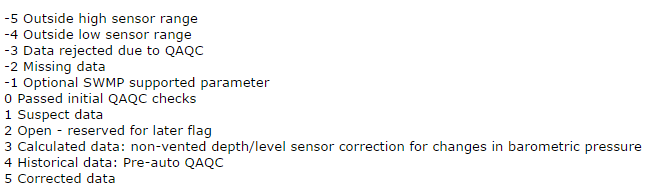
\includegraphics[width = 0.8\textwidth]{fig/qaqc_flags.png}}}
\end{frame}

%%%%%%
\begin{frame}[containsverbatim,shrink]{Retrieve SWMP data}
Raw data with QAQC columns
\begin{knitrout}\small
\definecolor{shadecolor}{rgb}{0.929, 0.973, 0.984}\color{fgcolor}\begin{kframe}
\begin{verbatim}
##         datetimestamp temp f_temp spcond f_spcond sal f_sal
## 1 2012-01-01 00:00:00   17   <0>      46     <0>   30  <0> 
## 2 2012-01-01 00:15:00   17   <0>      46     <0>   30  <0> 
## 3 2012-01-01 00:30:00   17   <0>      45     <0>   29  <0> 
##   do_pct f_do_pct do_mgl f_do_mgl depth f_depth cdepth
## 1     89     <0>       7     <0>      1    <0>       1
## 2     88     <0>       7     <0>      1    <0>       1
## 3     89     <0>       7     <0>      1    <0>       1
##   f_cdepth level f_level clevel f_clevel ph f_ph turb
## 1     <3>     NA   <-1>      NA       NA  8 <0>     2
## 2     <3>     NA   <-1>      NA       NA  8 <0>     4
## 3     <3>     NA   <-1>      NA       NA  8 <0>     4
##   f_turb chlfluor f_chlfluor
## 1   <0>        NA      <-1> 
## 2   <0>        NA      <-1> 
## 3   <0>        NA      <-1>
\end{verbatim}
\end{kframe}
\end{knitrout}
\end{frame}

%%%%%%
\begin{frame}[containsverbatim]{Organize SWMP data}
Data in red are `bad' QAQC flags
\begin{knitrout}
\definecolor{shadecolor}{rgb}{0.929, 0.973, 0.984}\color{fgcolor}

{\centering 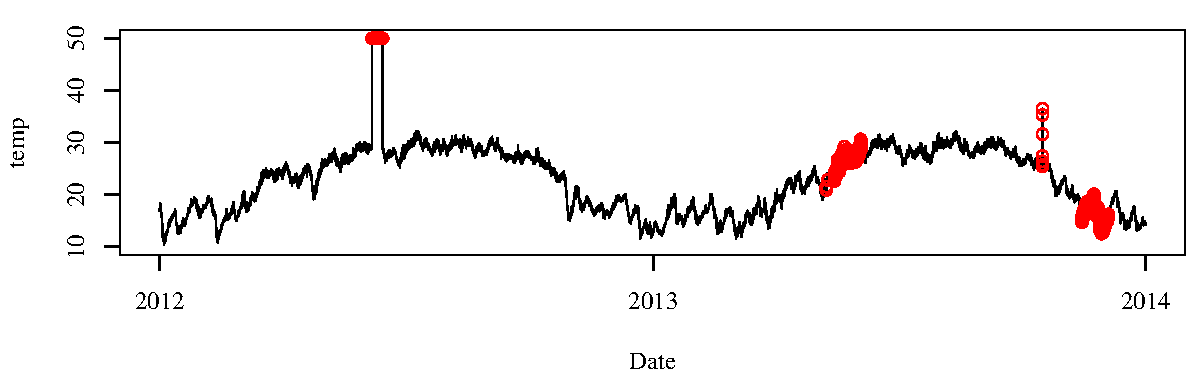
\includegraphics[width=0.9\textwidth]{fig/qaqc_ex1-1} 

}



\end{knitrout}
After using \texttt{qaqc} function
\begin{knitrout}
\definecolor{shadecolor}{rgb}{0.929, 0.973, 0.984}\color{fgcolor}

{\centering 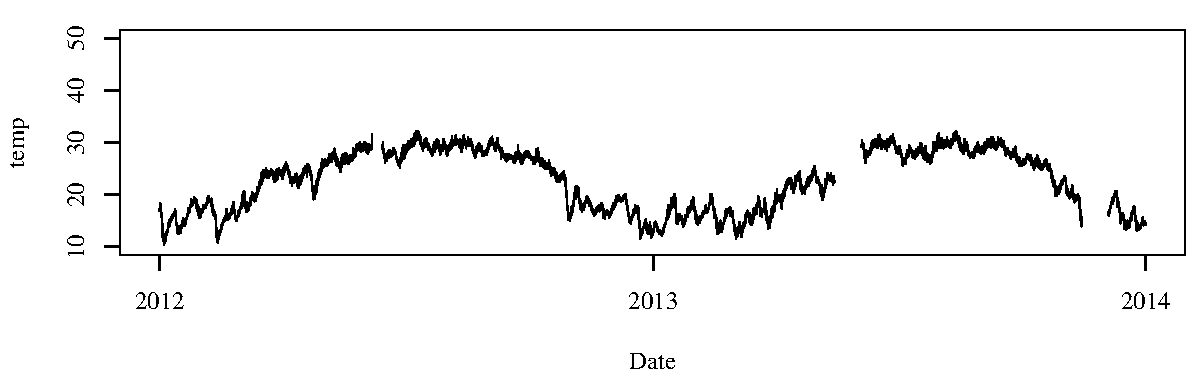
\includegraphics[width=0.9\textwidth]{fig/qaqc_ex2-1} 

}



\end{knitrout}
\end{frame}

%%%%%%
\begin{frame}[fragile]{How are data \Bigtxt{organized}?}
Example - we want to compare time series from different sites\\~\\
\begin{itemize}
\item Data may have arbitrary time steps that do not match between sites \\~\\
\item Date ranges may also differ \\~\\
\end{itemize}
The \texttt{comb} function addresses these issues! \\~\\
\begin{knitrout}
\definecolor{shadecolor}{rgb}{0.929, 0.973, 0.984}\color{fgcolor}\begin{kframe}
\begin{alltt}
\hlstd{> }\hlcom{# import all weather and wq data for Apalachicola}
\hlstd{> }\hlstd{met} \hlkwb{<-} \hlkwd{import_remote}\hlstd{(}\hlstr{'apaebmet'}\hlstd{)}
\hlstd{> }\hlstd{wq} \hlkwb{<-} \hlkwd{import_remote}\hlstd{(}\hlstr{'apacpwq'}\hlstd{)}
\end{alltt}
\end{kframe}
\end{knitrout}
\end{frame}

%%%%%%
\begin{frame}[fragile]{How are data \Bigtxt{organized}?}
\begin{knitrout}\small
\definecolor{shadecolor}{rgb}{0.929, 0.973, 0.984}\color{fgcolor}\begin{kframe}
\begin{alltt}
\hlstd{> }\hlkwd{dim}\hlstd{(met)}
\end{alltt}
\begin{verbatim}
## [1] 490847     11
\end{verbatim}
\begin{alltt}
\hlstd{> }\hlkwd{dim}\hlstd{(wq)}
\end{alltt}
\begin{verbatim}
## [1] 455808     13
\end{verbatim}
\begin{alltt}
\hlstd{> }\hlcom{# standardize time step to two hours}
\hlstd{> }\hlcom{# combine only overlapping time ranges}
\hlstd{> }\hlstd{dat} \hlkwb{<-} \hlkwd{comb}\hlstd{(wq, met,} \hlkwc{timestep} \hlstd{=} \hlnum{120}\hlstd{,} \hlkwc{method} \hlstd{=} \hlstr{'intersect'}\hlstd{)}
\hlstd{> }\hlkwd{dim}\hlstd{(dat)}
\end{alltt}
\begin{verbatim}
## [1] 56977    23
\end{verbatim}
\end{kframe}
\end{knitrout}
\end{frame}

%%%%%%
\begin{frame}[fragile]{How are data \Bigtxt{organized}?}
The combined dataset
\begin{knitrout}\small
\definecolor{shadecolor}{rgb}{0.929, 0.973, 0.984}\color{fgcolor}\begin{kframe}
\begin{verbatim}
##         datetimestamp atemp rh   bp wspd maxwspd wdir
## 1 2001-12-31 23:00:00     4 69 1017    4      NA  347
## 2 2002-01-01 01:00:00     3 75 1017    3      NA    9
## 3 2002-01-01 03:00:00     2 77 1018    3      NA  331
## 4 2002-01-01 05:00:00     1 82 1019    4      NA    0
##   sdwdir totpar totprcp totsorad temp spcond sal do_pct
## 1     NA      0      NA       NA   NA     NA  NA     NA
## 2     NA      0      NA       NA   12     37  24    104
## 3     NA      0      NA       NA   12     40  26     99
## 4     NA      0      NA       NA   11     42  26     98
##   do_mgl depth cdepth level clevel ph turb chlfluor
## 1     NA    NA     NA    NA     NA NA   NA       NA
## 2     10     2     NA    NA     NA NA    3       NA
## 3      9     2     NA    NA     NA NA    4       NA
## 4      9     2     NA    NA     NA NA    5       NA
\end{verbatim}
\end{kframe}
\end{knitrout}
\end{frame}

%%%%%
\begin{frame}{How are data \Bigtxt{analyzed}?}
Time series analysis can range from very general to very specific \\~\\
SWMPr functions include...\\~\\
\begin{columns}[t]
\begin{column}{0.45\textwidth}
\Bigtxt{General} \\~\\
\begin{itemize}
\item Approximate missing data
\item Smoothing with moving windows
\item Aggregate by time periods
\item Basic plots and histograms
\end{itemize}
\end{column}
\begin{column}{0.45\textwidth}
\Bigtxt{Specific} \\~\\
\begin{itemize}
\item Time series decomposition
\item Estimate net ecosystem metabolism
\item Aggregate metabolism
\item Summary plots of raw data
\end{itemize}
\end{column}
\end{columns}
\vspace{0.3in}
...or exit the SWMPr workflow and evaluate with other R packages
\end{frame}

%%%%%
\begin{frame}[fragile]{How are data \Bigtxt{analyzed}?}
Example: fill missing data \\~\\
\begin{knitrout}\scriptsize
\definecolor{shadecolor}{rgb}{0.929, 0.973, 0.984}\color{fgcolor}

{\centering 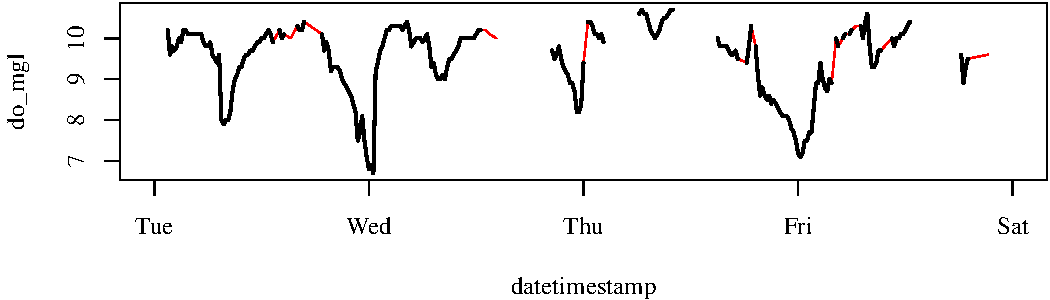
\includegraphics[width=0.85\textwidth]{fig//filled-1} 

}



\end{knitrout}
Example: smooth data \\~\\
\begin{knitrout}\scriptsize
\definecolor{shadecolor}{rgb}{0.929, 0.973, 0.984}\color{fgcolor}

{\centering 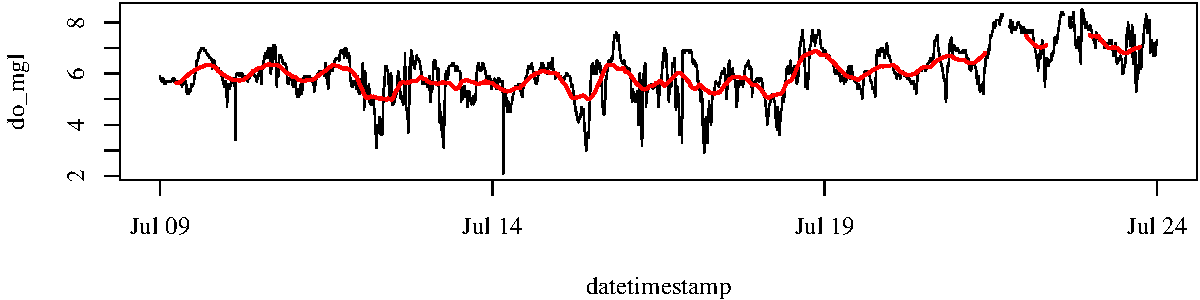
\includegraphics[width=0.85\textwidth]{fig//smooth-1} 

}



\end{knitrout}
\end{frame}

%%%%%%
\begin{frame}[fragile]{How are data \Bigtxt{analyzed}?}
Example: time series decomposition (chl-a at cbmocnut)\\~\\
\begin{knitrout}
\definecolor{shadecolor}{rgb}{0.929, 0.973, 0.984}\color{fgcolor}

{\centering 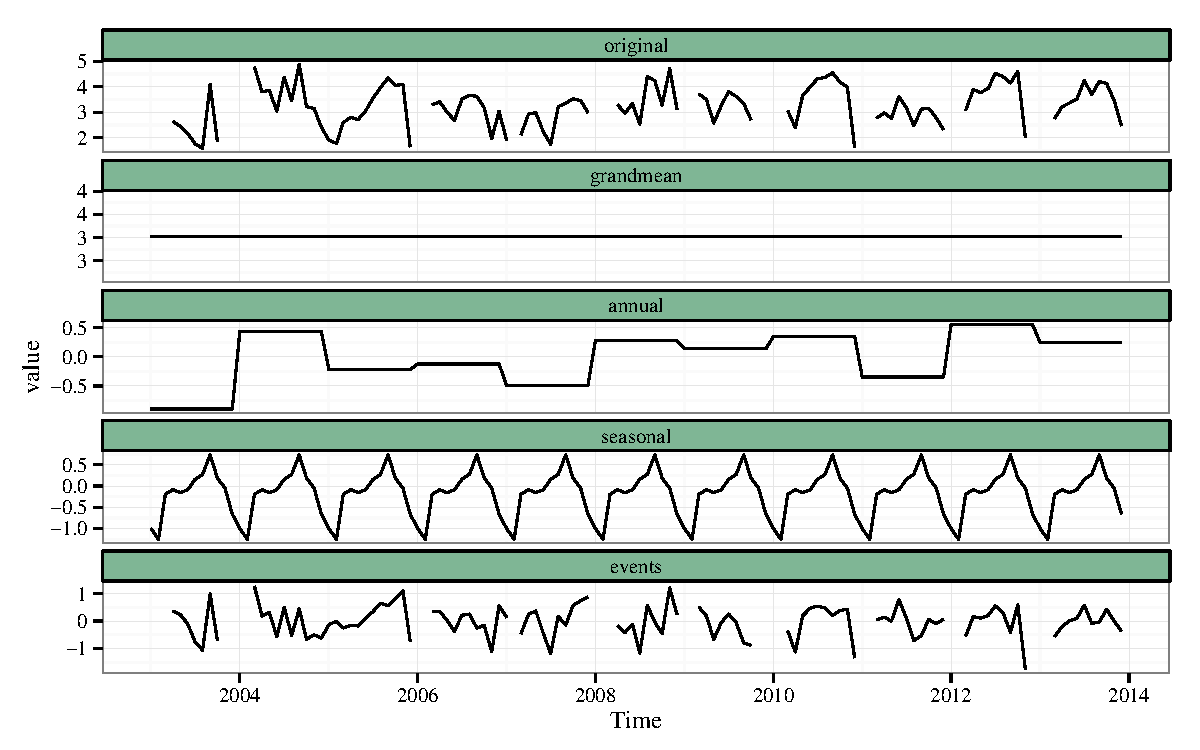
\includegraphics[width=0.85\textwidth]{fig/decomp_dep-1} 

}



\end{knitrout}
\end{frame}

%%%%%%
\begin{frame}[fragile]{How are data \Bigtxt{analyzed}?}
Example: estimate ecosystem metabolism

\begin{knitrout}
\definecolor{shadecolor}{rgb}{0.929, 0.973, 0.984}\color{fgcolor}

{\centering 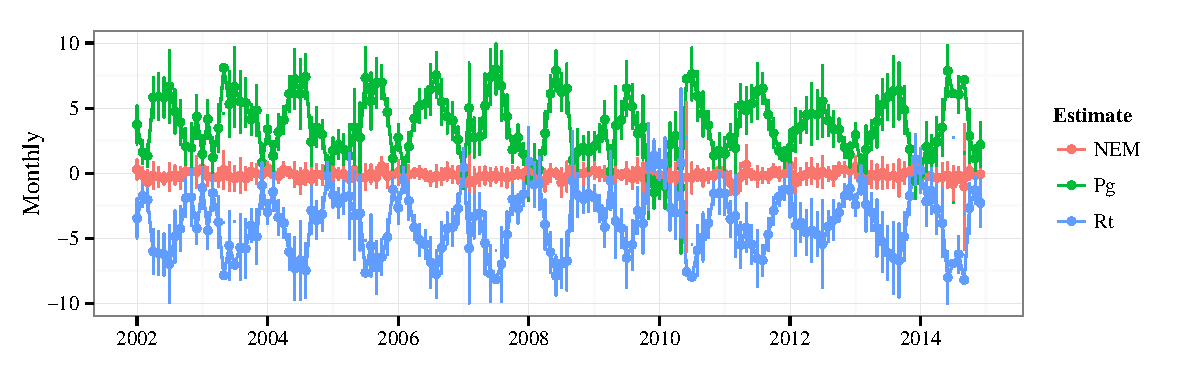
\includegraphics[width=0.95\textwidth]{fig//ecometab1-1} 

}



\end{knitrout}
\begin{knitrout}
\definecolor{shadecolor}{rgb}{0.929, 0.973, 0.984}\color{fgcolor}

{\centering 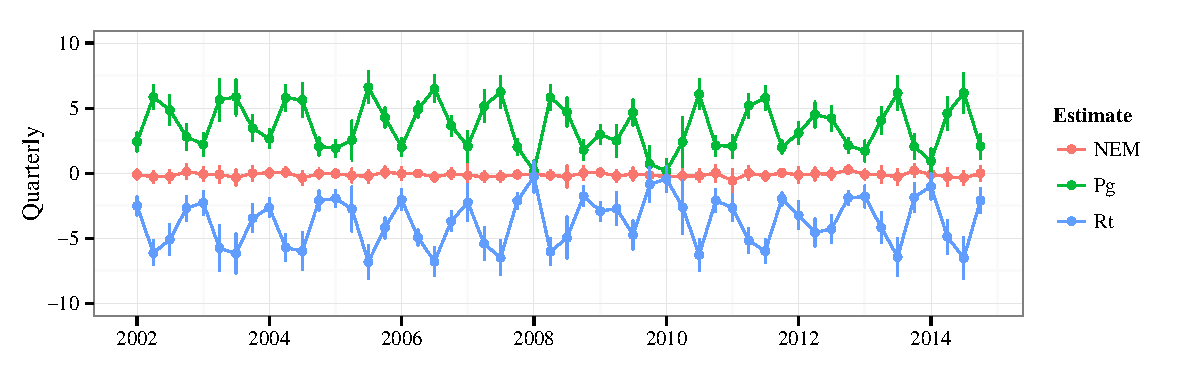
\includegraphics[width=0.95\textwidth]{fig//ecometab2-1} 

}



\end{knitrout}
\end{frame}

\section{SWMPr applications}

%%%%%%
\begin{frame}[fragile]{SWMPr applications}
The most common question - what is the change over time at my site? \\~\\
The functions in SWMPr can help, but it's easier to interact!\\~\\
Two online applications can help visualize trends \\~\\
\begin{columns}[t]
\begin{column}{0.45\textwidth}
\centerline{\Bigtxt{\href{https://beckmw.shinyapps.io/swmp_summary}{Summary plots}}}
\centerline{\fbox{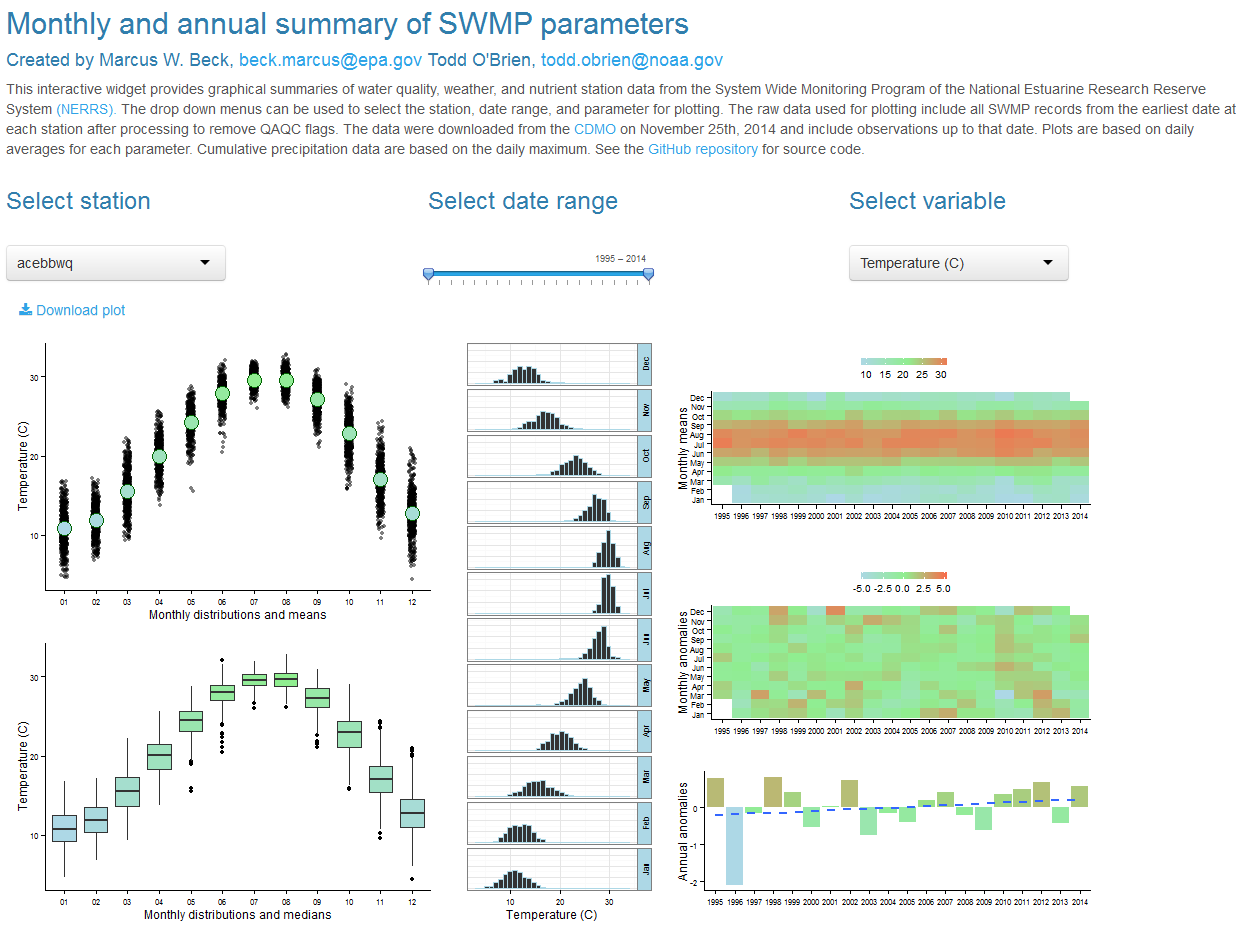
\includegraphics[width = 0.9\textwidth]{fig/swmp_summary.png}}}
\end{column}
\begin{column}{0.45\textwidth}
\centerline{\Bigtxt{\href{https://beckmw.shinyapps.io/swmp_comp}{Trends map}}}
\centerline{\fbox{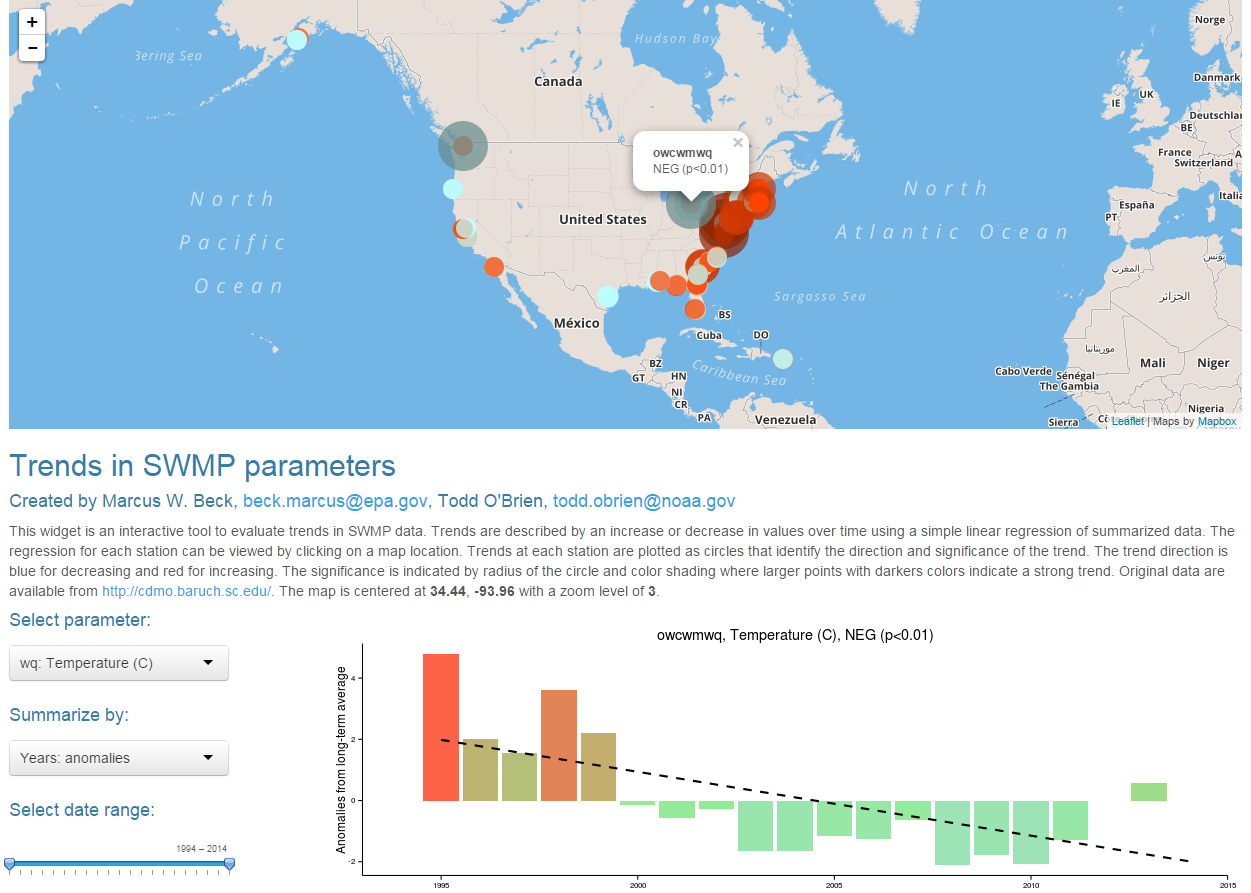
\includegraphics[width = 0.935\textwidth]{fig/swmp_comp.png}}}
\end{column}
\end{columns}
\end{frame}

%%%%%%
\begin{frame}[t]{SWMPr applications}
\href{https://swmprats.net}{SWMPrats.net}: \Bigtxt{S}ystem-\Bigtxt{W}ide \Bigtxt{M}onitoring \Bigtxt{P}rogram \Bigtxt{R}esources for the \Bigtxt{A}nalysis of \Bigtxt{T}ime \Bigtxt{S}eries \\~\\
\centerline{\fbox{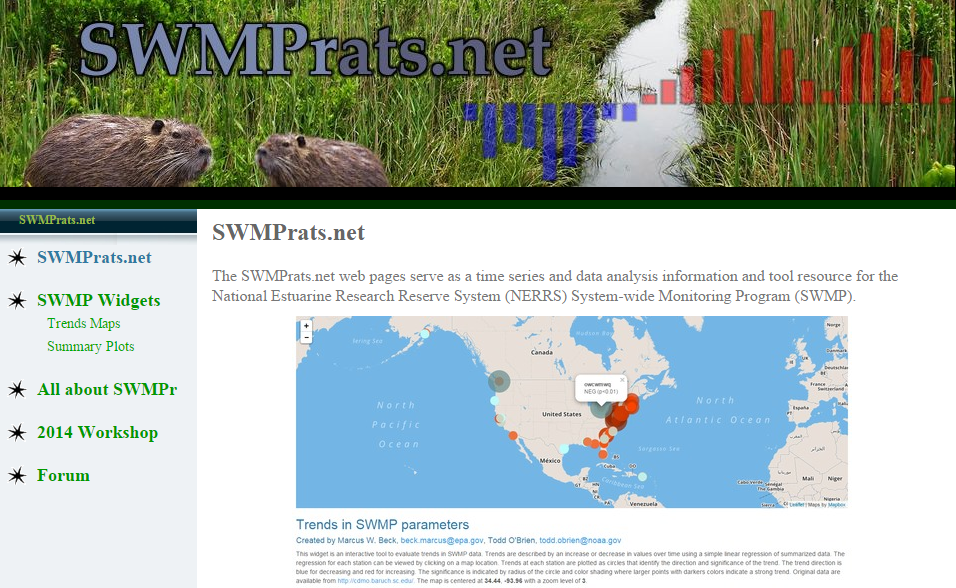
\includegraphics[width = 0.75\textwidth]{fig/swmprats_home.png}}}
\end{frame}

%%%%%%
\begin{frame}{SWMPr applications}
The SWMPr package provides an R-centric approach to \Bigtxt{retrieve}, \Bigtxt{organize}, and \Bigtxt{analyze} estuary data \\~\\
A new program, but already seeing heavy use:\\~\\
\begin{itemize}
\item SWMPr downloaded 306 times from R network (as of April 30) \\~\\
\item Apps have been used 347 hours (as of April 30) \\~\\
\end{itemize}
SWMPr is meant to \Bigtxt{augment}, not replace, existing data management programs (i.e., CDMO web services) \\~\\
Deals with lots of the heavy lifting with large, unrefined datasets \\~\\
\end{frame}

\section{Novel applications}

%%%%%%
\begin{frame}{Novel applications}
Similarities between... \\~\\
\begin{columns}[t]
\begin{column}{0.45\textwidth}
\Bigtxt{SWMP}\\~\\
\begin{enumerate}
\item Continuous wq and weather data
\item Data from multiple sources - individual reserves
\item Interested end users - NOAA, NERRS RCs/managers
\end{enumerate}
\end{column}
\begin{column}{0.45\textwidth}
\Bigtxt{Stream networks} \\~\\
\begin{enumerate}
\item Continuous pressure/temperature data
\item Data from multiple sources - states/tribes
\item Interested end users - EPA, states/tribes
\end{enumerate}
\end{column}
\end{columns}
\vspace{0.3in}
The SWMPr approach is generic enough to be adapted to other applications...
\end{frame}

%%%%%%
\begin{frame}{Novel applications}
Some questions/comments... \\~\\
\begin{itemize}
\item Distinction between data management systems vs data analysis tools, not mutually exclusive but there are key differences \\~\\
\item Data format and availability (STORET, WQX, WQP) \\~\\
\item Desired products - data processing vs data analysis/viz \\~\\
\item General questions to address - climate change...
\end{itemize}

\end{frame}

\end{document}
